\documentclass{article}
\usepackage[utf8]{inputenc}

\title{Cosmological Evidences of Dark Matter through the CMB}
\author{Lorenzo Speri}
\date{}
%\usepackage{hyperref}
\usepackage{natbib}
\usepackage{graphicx}
% ---- Maths -------
\usepackage{amsmath}
\usepackage{amsthm}
\usepackage{physics}
% ---- Links -------
%\usepackage{hyperref}
% citation color
\usepackage[colorlinks=true,citecolor=blue]{hyperref}
% for twnsore
\usepackage{tensind}
\tensordelimiter{:}


%  ---- my commands -------
\newcommand{\bea}{\setlength{\jot}{10pt}\begin{eqnarray*}}
\newcommand{\eea}{\end{eqnarray*}}
\newcommand{\beq}{\begin{equation}}
\newcommand{\eeq}{\end{equation}}
\newcommand{\bpsi}{\bar{\psi}}
\newcommand{\dslash}{\slashed{\partial}}
\newcommand{\Dslash}{\slashed{D}}
\newcommand{\Lagr}{\mathcal{L}}
\newcommand{\cpp}{\texttt{C++} } 
\newcommand{\mpi}{\texttt{MPI} } 
\newcommand{\de}{\nu}
\newcommand{\T}{\text{TT}}
\newcommand{\h}{\mathscr{H}}
\newcommand{\ten}{\mathscr{T}}

\begin{document}

\maketitle


\section{Introduction}
Many astronomical and cosmological observations suggest that there is a missing form of matter that interacts gravitationally. 
In order to explain such observations, scientists have proposed the existence of Dark Matter, a new form of matter that does not interact electromagnetically but gravitationally.
However, the fundamental nature of Dark Matter is not well understood yet, and whether Dark Matter is truly a new form of matter or the effect of new laws of gravity is still matter of debate.\\
One of the most compelling evidence for the existence of Dark Matter comes from the analysis of the Cosmic Microwave Background (CMB).
In this paper we explain how the  analysis of the CMB is linked to the energy-matter content of our Universe, and, within this framework, we study the role of Dark Matter.
The aim of this paper is to give a short and concise overview of the cosmological evidence of Dark Matter given by the observations of the CMB.
We are interested in providing few but fundamental ingredients to understand the importance of the CMB for Dark Matter to a reader that is not familiar with the topic.
\\
 

\subsection{The Cosmic Microwave Background in few lines}


The Cosmic Microwave Background is the electromagnetic radiation coming from the hot plasma of the early stages of the Universe.
When the Universe, made of hot plasma, reached a temperature low enough to form stable hydrogen $e^- + p^+  \rightarrow H + \gamma$ the number density of the free electrons dropped, causing the Thomson scattering $e^- + \gamma  \rightarrow e^- + \gamma$ to be inefficient and the photons to decouple. They have since streamed freely through the universe and are today observed as the Cosmic Microwave Background \citep{LecturesPdf}.\\

-practical Motivation for studyinbg the cmb: nice spectrum black body spectrum: physics well know, very intense radiation\\
which info can we get from the cmb: Big bang, maater and energy content of the universe---dark matter is a big part of the matter content it influenced the spectrum  of the CMB ---- so it played a role.\\
-\textbf{structure of the paper} \\
--The experimental results from the observations of the Cosmic Microwave Background provide important details about energy-matter content of the Universe.


%The recent measurements of the Cosmic Microwave Background (CMB) radiation allowed us to infer the presence of Dark Matter in the Universe. In this summary we will explain qualitatively how the presence of Dark Matter influences the CMB anisotropies.

\section{From the Discovery of the CMB to the Planck mission}

\begin{figure}
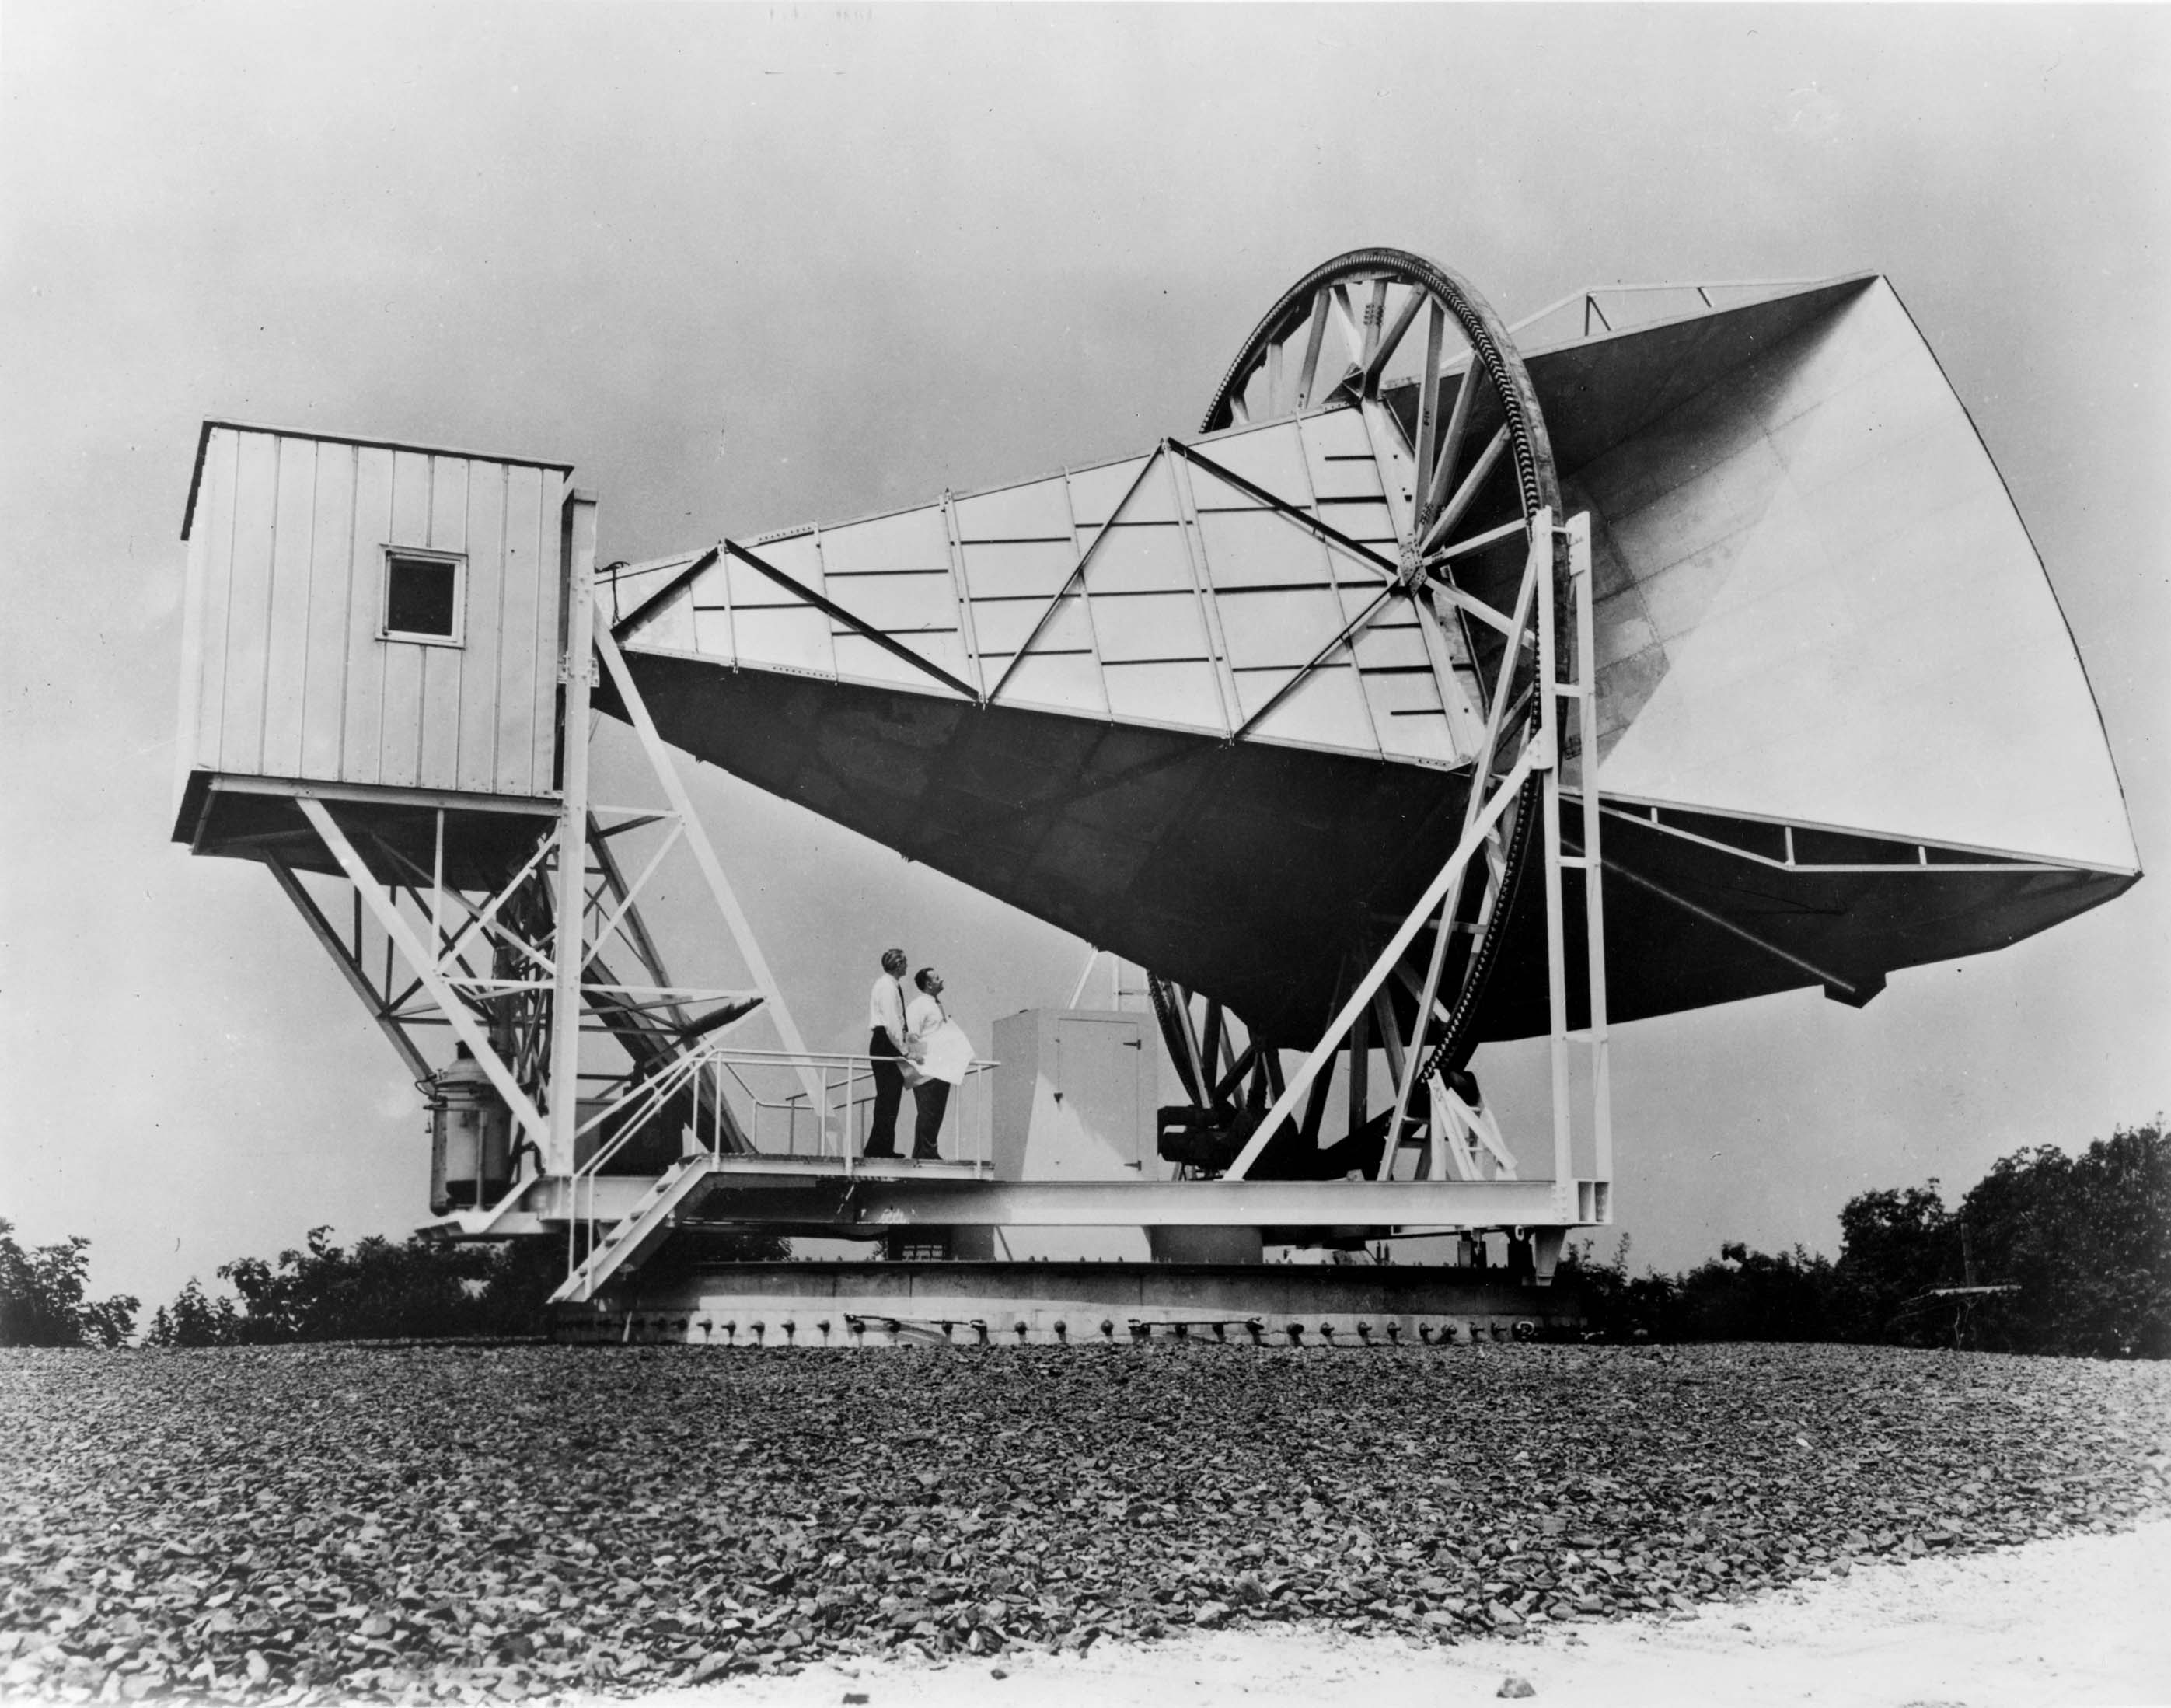
\includegraphics[width=\textwidth]{Horn_Antenna.jpeg}
\caption{The 15 meter Holmdel horn antenna at Bell Telephone Laboratories in Holmdel, New Jersey.
(By NASA - Great Images in NASA Description, Public Domain, \url{https://commons.wikimedia.org/w/index.php?curid=6463768})}
\end{figure}

In 1965 Arno Penzias and Robert Wilson published the paper: \emph{A measurement of excess antenna temperature at
4080 Mc/s}, where they reported the measurements of an isotropic, unpolarized, and free from seasonal variations excess noise temperature
\citep{penziasMeasurementExcessAntenna1965}. 
When Penzias and Wilson first measured serendipitously this strong signal, they did everything they could think of to reduce “noise” in their system. 
They even shooed away a pair of pigeons that had roosted in the antenna and cleaned up they later called “the usual white dielectric” generated by pigeons \citep{RydenIntroCosmoPdf}.
However, the signal remained. 
Robert Dicke and his research group at Princeton University explained such signal as the relic of an early, hot, dense, and opaque state of the universe\footnote{the existence of the cosmic background radiation had actually been predicted by the physicist George Gamow and his colleagues in 1948} \citep{bucherPhysicsCosmicMicrowave2015}
. \\
This discovery of the CMB created a big excitement and a new era of cosmology began.
Measuring the CMB spectrum and its deviation from the black body spectrum was the new challange.
Many experimental efforts have been carried out to measure accurately the fluctuations of Cosmic Microwave Backgrund from its average temperature $T = 2.7$ K, we will discuss only few of them.
\\
First of all, the photons of the CMB can be absorbed by the Earth's atmosphere, because the energy per CMB photon (approximately $\sim 6 \times 10 ^{-4}$ eV) is comparable to the energy of vibration or rotation for a small molecule (of water for instance). In fact, microwaves with wavelengths shorter than $\lambda \sim 3$ cm are strongly absorbed by water molecules \citep{RydenIntroCosmoPdf}.
This problem could be overcomed by observing the CMB in different bands and from locations where the humidity is low.
However, the best way to meseaure the CMB spectrum is to use satellites.\\
The first sattellite that was launched to observe the CMB was COBE. 
It did provide a convincing first detection of the CMB anisotropy, and it played a crucial role in determining the viability of the different cosmological models at that time.
\\
After that, WMAP and PLanck space missions  increased the accuracy of the measurements Figure (\ref{cobe_wmap_planck}).
Nevertheless the satellites improved their accuracy, many other sources of noise were encountered such as the light coming from the center of our galaxy, other stars and other objects in the universe, in addition to the relative motion of the satellite with respect to the CMB (Figure (\ref{cobe_map})).\\
Finally, observations and statistical analysis showed that the CMB spectrum is close to a black body spectrum up to fluctuations of order of $10^{-5}$ K (Figure (\ref{cobe_blackbody})).\\
% maybe last sentence in the introduction with the image

\begin{figure}
\centering
    \textbf{Cosmic Microwave Background  Spectrum}\par\medskip
\centering
   {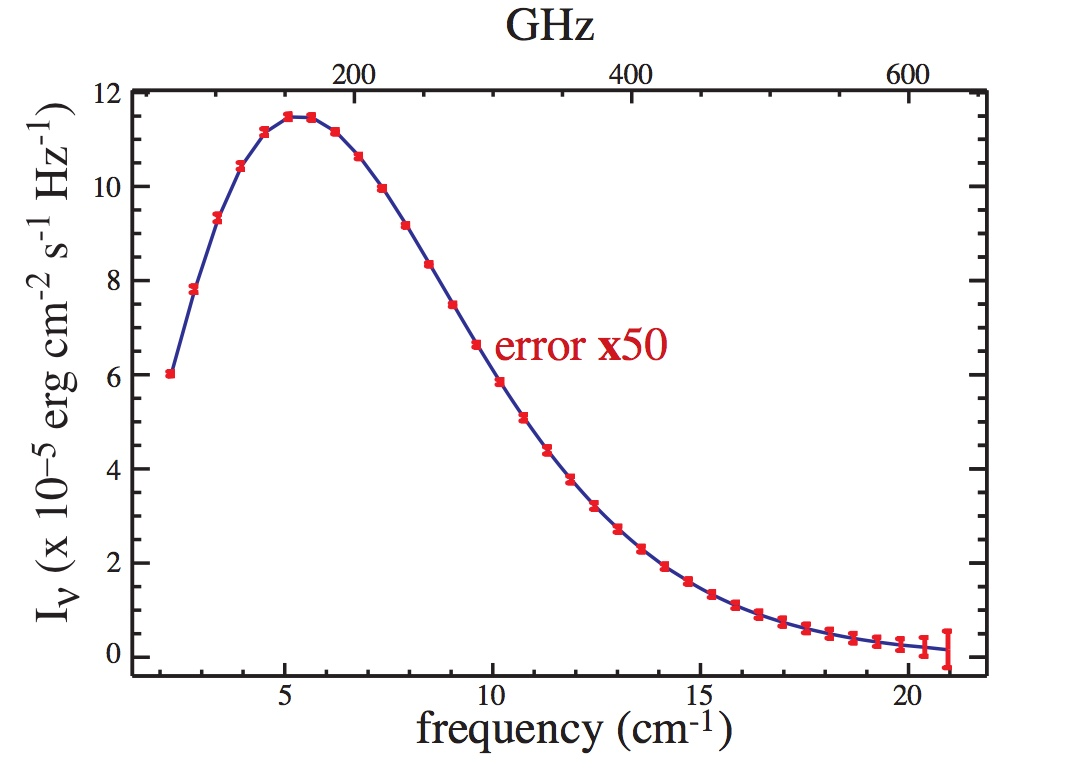
\includegraphics[height=8cm]{blackbody}}
\caption{}
\label{cobe_blackbody}
\end{figure}


\begin{figure}
\centering
    \textbf{The Cosmic Microwave Background anisotropies measured by COBE, WMAP and Planck}\par\medskip
\centering
   {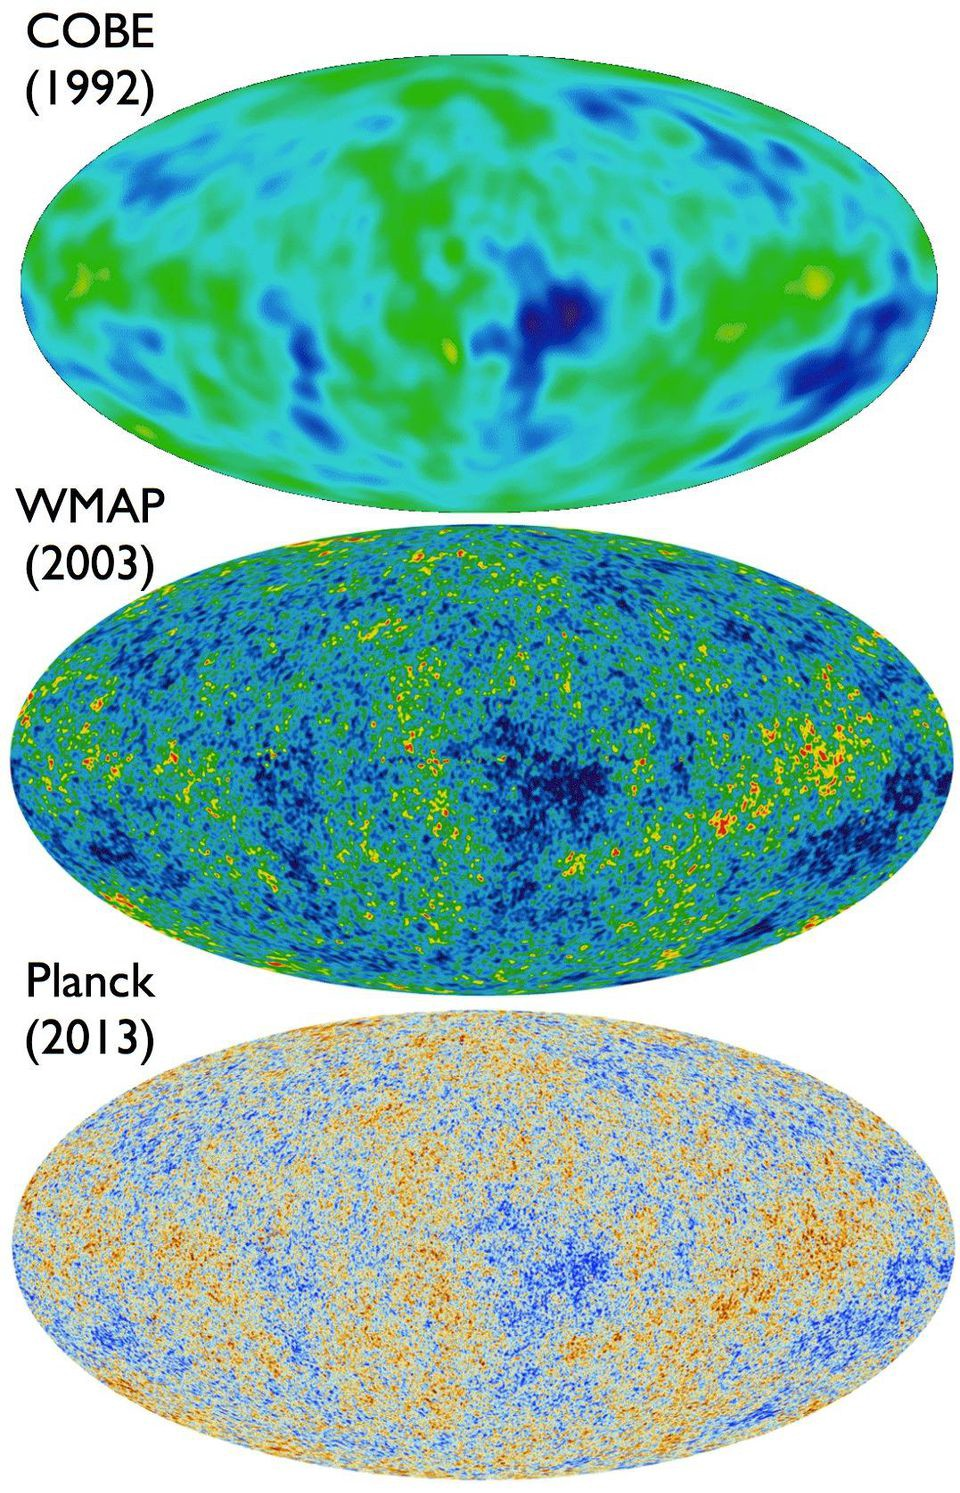
\includegraphics[width=.45\textwidth]{cobe_wmap_planck.jpg}}


\caption{The COBE, WMAP and Planck missions measured the CMB anisotropies with increasing accuracy. COBE, the first CMB satellite, measured fluctuations to scales of 7$^\circ$. WMAP was able to measure resolutions down to 0.3$^\circ$ in five different frequency bands, with Planck measuring all the way down to just 5 arcminutes (0.07$^\circ$) in nine different frequency bands in total.  (NASA/COBE/DMR; NASA/WMAP SCIENCE TEAM; ESA AND THE PLANCK COLLABORATION)}
\label{cobe_wmap_planck}
\end{figure}


\begin{figure}
\centering
    \textbf{Orbits of different  configurations of BBH}\par\medskip
\centering
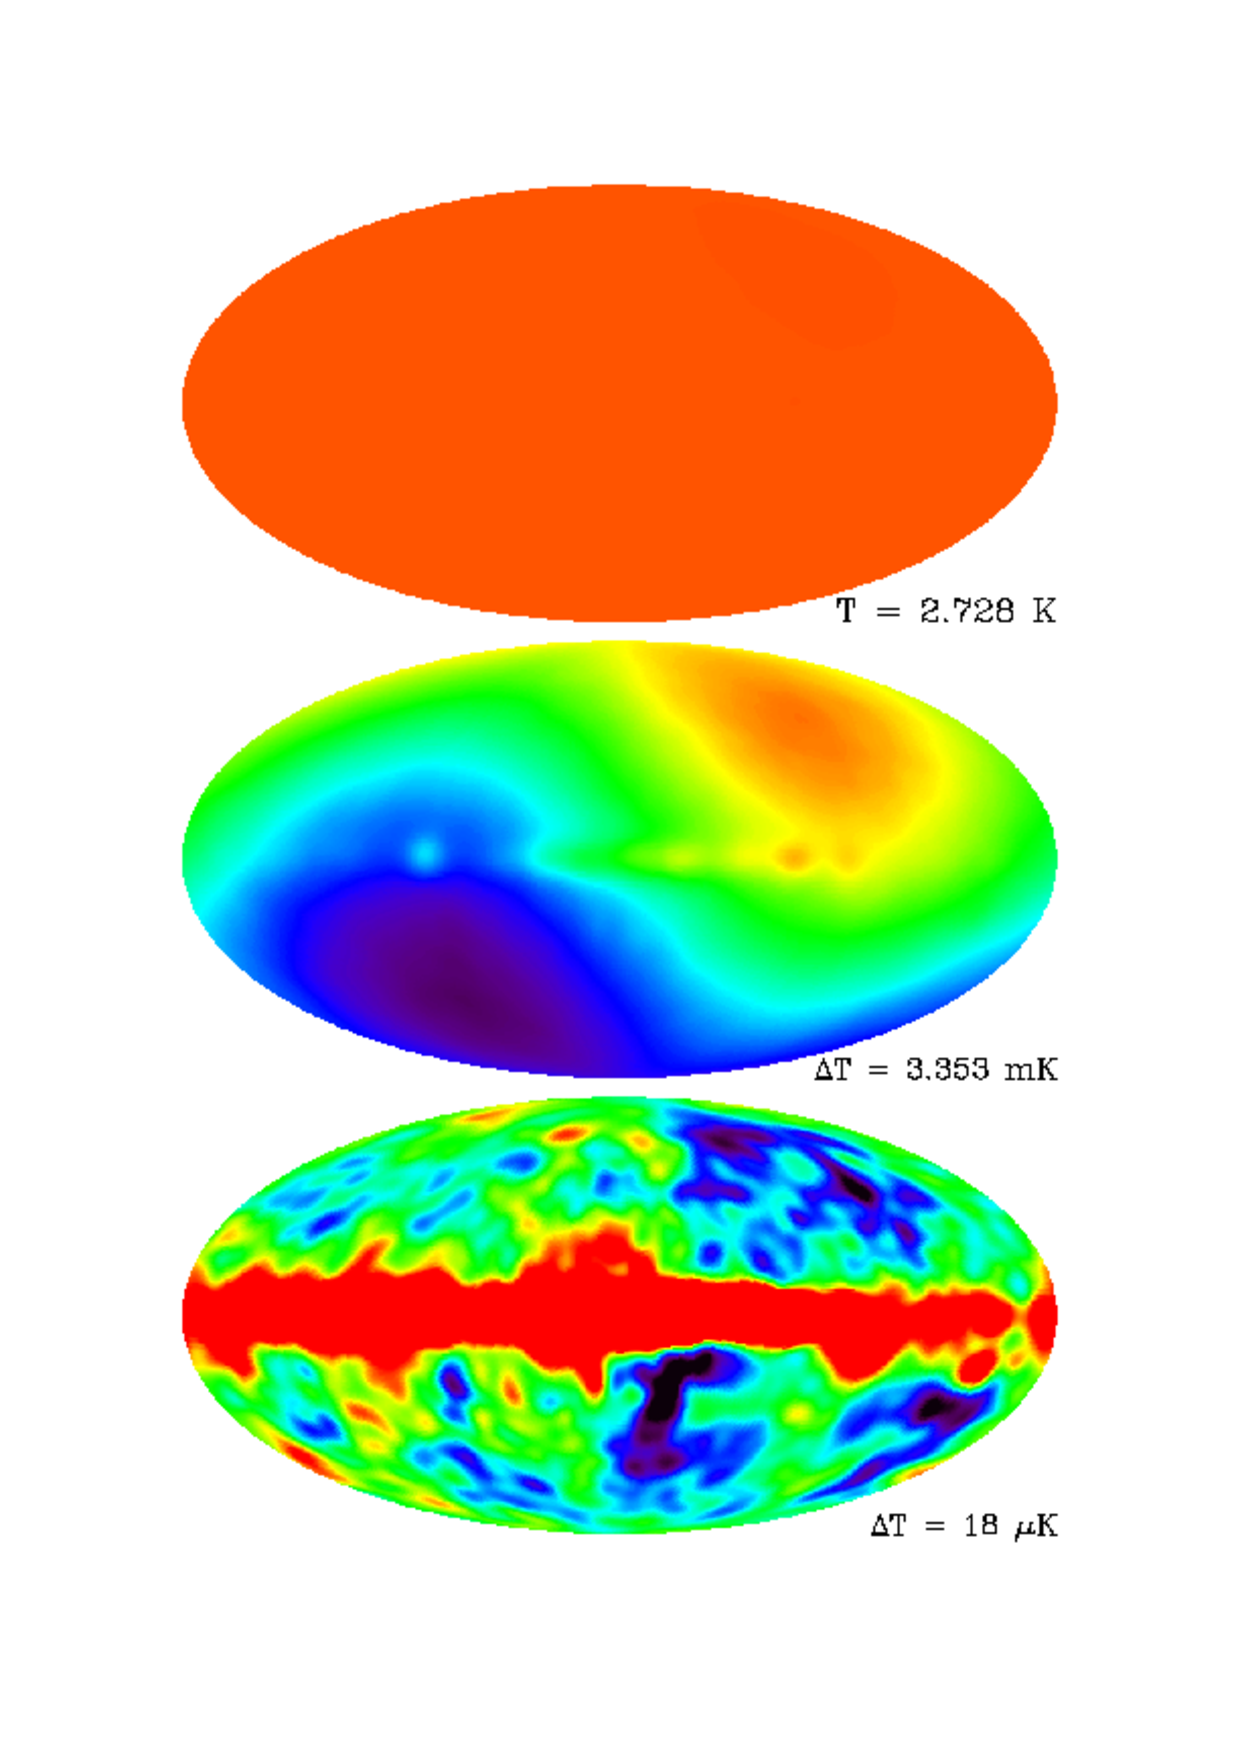
\includegraphics[scale =0.3]{mono_di_cobe}
\caption{The microwave sky as seen by the COBE DMR (differential microwave radiometer) instrument. The top panel shows the microwave sky as seen on a linear tem- perature scale including zero. No anisotropies are visible in this image, because the CMB monopole at 2.725K dominates. In the middle panel, the monopole component has been subtracted. Apart from some slight contamination from the galaxy near the equator (corre- sponding to the plane of our Galaxy), one sees only a nearly perfect dipole pattern, owing to our peculiar motion with respect to the rest frame defined by the CMB. In the bottom panel, both the monopole and dipole components have been removed. Except for the galactic contamination around the equator, one sees the cosmic microwave background anisotropy along with some noise. (Credit: NASA/COBE Science Team)}
\label{cobe_map}
\end{figure}

\newpage


\section{Content of the Universe} 
It is often said that our Universe is made up of $68.8$\% of Dark Energy, and $26.8 $\% by Dark Matter and $4.9 $\% of ordinary matter, but what do we really mean by that?\\
In this section we explain where the components of our Universe (Dark Matter, baryonic matter, Dark Energy, curvature)  arise from and how they are related with each others. 
The assumptions and the theoretical framework that we are going to explain will be then used to analyze the observations of the CMB.\\
We assume that the observable properties of the Universe are isotropic and there is not a preferred direction. 
Therefore, the Universe is assumed to be homogenous and isotropic at enough large scales $> 100$ Mpc, at least up to the observable universe.\\
Another important assumption is that there exists a class of observers at rest with respect to the Cosmic Microwave Background \citep{bartelmannStandardModelCosmology}.
Let us clarify this concept. 
After subtracting the average temperature of the CMB from its spectrum, a moving observer with respect with the CMB will see a dipole pattern, where the blue-shifted photons come from the direction the observer is moving toward to and the red-shifted photons from the opposite direction.
Since Earth is not at rest with respect to the CMB, the satellite COBE measured the dipole pattern showed in the second panel in Figure (\ref{cobe_map}).\\
Given these assumptions, the most general metric $g_{\mu \nu}$ satisfying homogeneity and isotropy is the Friedmann–Lemaître–Robertson–Walker (FLRW) metric written here in terms of the invariant geodesic distance $\dd s ^2 = g_{\mu \nu} \dd x^{\mu} \dd x^{\nu}$:
\begin{equation}
\label{metric}
\dd s ^2 = -\dd t^2 + a^2 (t) \qty( \frac{1}{1-k \, r^2} \dd r^2 + r^2 \dd \Omega ^2 )  
\end{equation}
where $k$ is the spatial curvature and $a(t)$ is the scale factor (we set the light speed $c=1$).
Notice that the FLRW metric has $g_{0 i}=0$ due to the isotropy.
\\ % comments on the redshift, metric, what spatially flat means
If we assume the correctnes of the General Theory of Relativity, we can use the Einstein's field equations
\begin{equation}
\label{einstein_eq}
R_{\mu \nu} - \dfrac{1}{2} R \, g _{\mu \nu} + \Lambda g_{\mu \nu}= 8 \pi G \, T_{\mu \nu}
\end{equation}
in order to evolve the FLRW metric.
The Einstein's field equations relate how the geometry of spacetime (left hand side) changes with the presence of masses and energy (right hand side).
The most general fluid consistent with the assumption of homogeneity and isotropy is a perfect fluid, one in which an observer comoving with the fluid would see the universe around it as isotropic \citep{garcia-bellidoAstrophysicsCosmology2000}. Therefore, the energy-momentum tensor $T_{\mu \nu}$ can be written as
\begin{equation}
\label{energy-momentum-tensor}
T^{\mu \nu } = (p + \rho)u ^{\mu} u^{\nu}+p g^{\mu \nu} 
\end{equation}
where $\rho$ and $p$ are, respectively, the mass density and the pressure of the fluid.\\
Solving (\ref{einstein_eq}) for $\mu= 0=\nu$ using the above definition (\ref{energy-momentum-tensor}), gives us the Friedmann equation:
\begin{equation}
\label{firedmann_eq}
\begin{split}
H^2 = \qty(\frac{\dot{a}}{a})^2 = \dfrac{8 \pi G}{3} \rho -\dfrac{k}{a^2} + \frac{\Lambda}{3}
\end{split}
\end{equation}
where $\dot{a}$ is the time derivative of the scale factor.\\
And the conservation of energy momentum tensor $\nabla_\mu T^{\mu 0} =0 $ becomes:
\beq
\label{energy_cons}
\dv[]{}{t}\qty(\rho a^3) + p \dv[]{}{t} \qty(a^3)  = 0
\eeq
Solving for radiation $\rho = p/3$
\[
\dot{\rho}  + 4 \frac{ \dot{a}}{a} \rho =0
\]
 And solving for matter $\rho << p$
 \[
 \dot{\rho}  + 3 \frac{ \dot{a}}{a} \rho =0
 \]
Solving this for matter $\rho_m << p_m$ (or \emph{dust}) and for radiation $\rho_r = p_r/3$ gives
\begin{equation}
\begin{split}
\rho_m = \rho_{m 0} a^{-3} \hspace{1.5cm} \rho_r = \rho_{r 0} a^{-4} \notag
\end{split}
\end{equation}
where $\rho_{m 0}$ and $\rho_{r 0}$ are the matter density and radiation density evaluated today $t = t_0$, $a(t_0) = a_0 =1$.\\
We now rewrite equation (\ref{firedmann_eq}) as
\begin{equation}
H ^2 = H_0 ^2 \qty[
\dfrac{8 \pi G}{3 H_0 ^2} \rho_{m 0} a^{-3}+
\dfrac{8 \pi G}{3 H_0 ^2} \rho_{r 0} a^{-4}+ 
\dfrac{-k}{H_0 ^2} a^{-2} + \dfrac{\Lambda}{3 H_0 ^2}
] \notag
\end{equation}
where we defined $H_0 = H(t_0)$.\\
\beq
\Omega_\Lambda = \dfrac{\Lambda}{3} \qquad \Omega_k = -  \dfrac{k}{H_0 ^2} \qquad
\Omega_m = \dfrac{8 \pi G}{3 H_0 ^2} \rho_{m 0} \qquad \Omega_r =\dfrac{8 \pi G}{3 H_0 ^2} \rho_{r 0}
\eeq
evaluating the Friedmann equation (\ref{firedmann_eq}) today we obtain the cosmic sum rule
\begin{equation}
\label{cosmic_rule}
\Omega_{\Lambda} + \Omega_{m} + \Omega_k + \Omega_{r} = 1
\end{equation}







\section{Acoustic Oscillations}
The Cosmic Microwave Background is the image of the fluctuations of a dense and hot fluid made of matter (baryonic and dark) and radiation.
Before the release of the CMB at $z > 1100$ the electromagnetic radiation is firmly coupled (both energetically and kinetically) to the baryons and it is possible to describe the behavior of such a system by using the equations of relativistic hydrodynamics and the Einstein's field equations (\ref{einstein_eq}).
The full general-relativistic description of the photon-matter fluid requires a long derivation that can be found here [BAUMANN].\\
So, we show how the acoustic oscillations arise from a simple non-relativistic model of a ideal fluid under the effect of a gravitational potwntial $\phi$.
We assume that there is a set of fields \\
Derivation from Bartelmann

\begin{itemize}
\item hydrodynamics \citep{huLectureNotesCMB2008}
page 14 eq 49 to page 17 eq 71\\
skip doppler effect
\item gravito acoustic oscillations page 19 up to eq 82 , justify briefly constant potential in page 20
% if stress perturbations are negligible compared with density perturbations ( δp ≪ δρ ) then the potential will remain constant in periods where the background equation of state p/ρ is constant
\item page 20 and 21 up to eq92 important comment 
%The consequence is that overdense regions where Ψ is negative (potential wells) are cold spots in the effective temperature.
\item baryonic effect
\end{itemize}

\section{Comments on the results and plots of the CMB spectrum}







\section{Conclusion}
nn
\citep{padmanabhanDetectingDarkMatter2005}



\bibliographystyle{plain}
\bibliography{dark_1}
\end{document}
